\section{Learning Classifier Systems}
\label{section:learning-classifier-systems}

The field of LCSs, introduced in the 1970ies \cite{Hol75,Hol76,HR78}, is one of the most active and best-developed form of genetic based machine learning \cite{Kov02a,KL00,Lan08}. As mentioned above, much of LCS's theory is inherited from the reinforcement learning literature. % The following section provides a brief overview what an LCS is. 
Hence, LCSs are rule-based on-line learning systems that combine nature-inspired optimization heuristics and reinforcement learning techniques to learn appropriate actions for any input they get \cite{Wil95}. They are applicable to any problem, where a numerical reward reflecting the quality of an action can be obtained. The core component of a LCS is its \emph{rule base} that contains rules (called \emph{classifiers}) consisting mainly of a condition, an action, and a prediction value. The selection of an appropriate action for a given input is a two-step process. From the rule base of all classifiers a subset called \emph{match set} is computed, which contains all classifiers whose condition matches the current input. Then, for all distinct actions present in the match set, the average prediction of all classifiers advocating the same action is calculated and an action is selected (randomly or depending on the average prediction). Classifiers that advocate that action form the \emph{action set}.
%After that, the action with the highest average prediction is selected for execution (called \emph{best selection}) and all classifiers in the match set advocating that action form the \emph{action set}. An alternative of \emph{best selection} is \emph{tournament selection} \cite{Butz2003}, where the probability of being selected depends on the average prediction value. 
Finally, the reward received from the environment is subsequently used to update the prediction values of all classifiers in the corresponding action set.

Classifiers forming the rule base are created in two ways: Whenever the match set is empty, classifiers are inserted into the rule base by a process called \emph{covering}, which consists of a condition that matches the current input, a random action, and a default prediction value. Furthermore, a randomized \emph{evolutionary component} occasionally selects % relatively 
good classifiers to be the parent individuals for a reproduction cycle. Crossover and mutation are applied to copies of the parents to form offspring, which is inserted into the rule base. A variety of different LCS implementations has been proposed (cf.~\cite{Kov02a}), many are based on Wilson's XCS \cite{Wil95} system, which is an implementation that maintains separate prediction and fitness values and where the fitness of a classifier is based on the \emph{accuracy} of the prediction reward.  
% While Wilson originally used a binary input encoding for XCS, different approaches to represent real-valued inputs have been examined (e.\,g., \cite{DAL05a}). % (\eg, \cite{DAL05a,SB03,Wil00a}).

% The architecture of an LCS is simple to study and the knowledge is encoded and stored in so-called \emph{classifiers}. These classifiers consist of a condition part, which is matched against the input from the environment, an action part, and some kind of fitness or strength value.

% The strength value is used to decide, which classifier should be chosen if more than one classifier matches the current input. The encoding of conditions is done in such a way that different levels of \emph{generality} are possible, hence the range of input values each classifier matches against may vary from a single point to the entire search space. In a step that is called \emph{rule discovery} new classifiers are generated using genetic operators, like crossover and mutation, on existing classifiers, changing both condition and action. Furthermore, every time no classifier matching the current input is available, one or more classifiers with a matching condition and randomly chosen action are created (this is called \emph{covering}).

% After a classifier has been generated, the system has to determine its strength value. Every time a classifier's action is chosen, the strength value of this classifier is updated using some objective function. 

In certain problems (see Section~\ref{subsection:single-step-vs-multi-step-problems}), the environment's reaction to an action executed by an LCS is not instantaneous. Thus, further reinforcement learning cycles are required to build up an optimal (local) reward function (see Section~\ref{subsection:learning-markov}). Also, more complex scenarios with \emph{aliasing positions} require additional handling like an internal memory (see Section~\ref{subsection:non-markov-environments}). In dynamic predator/prey scenarios, additional measures are required, as discussed in the following.

% The simplest way to increase performance would be to try and find classifiers, which maximize the objective function's value. Another approach more suitable for complex problems is the use of three distinct components as \emph{strength value}: The prediction $p$ of the objective function's value after this classifier's action has been executed, the average error of this prediction $\epsilon$, and a fitness value $F$ computed from this prediction error. The prediction is used to choose an action for execution: The classifier with best prediction, weighted by its fitness, is likely to result in best performance. Furthermore, the fitness is used to find classifiers suitable as input for the generation of new classifiers using genetic operators. The goal is to represent the entire search space with as few classifiers as possible while keeping only those that are more \emph{accurate} in their prediction. This approach is realized in \emph{XCS, the eXtended Classifier System} \cite{Wil95}, which is used within this paper and described in \cite{But00,BW02}.

\subsection{Single-Step vs.\ Multi-Step Problems}
\label{subsection:single-step-vs-multi-step-problems}

Literature about LCSs could be divided into \emph{single-step} and \emph{mul\-ti-step} approaches. This separation bases on how to solve the reinforcement learning problem and addresses a design decision, which has to be taken when implementing an LCS. It refers to the question, \emph{when} a reinforcement signal (reward) is achieved from the environment and \emph{how} this reward is distributed on the past action(s). 

In \emph{single-step} environments having a single (centralized) learning instance, the external reward is received on every time step and the environmental input for each time step has completely been independent of the prior time step. % in the case of environments with only a single entity with an LCS.
When a decision is made, the reinforcement is directly received and measures the quality of the decision. Single-step environments generally involve categorization of data examples. A typical single-step benchmark problem is the \emph{boolean multiplexer problem} \cite{BKLW04,Wil95}. 

In \emph{multi-step} environments, the external reward may not necessarily be received on any time step, since the environmental input on a time step depends on at least the prior input and the system's last action. Typical multi-step environments are known as sequential environments or so-called \emph{Maze} problems ( e.\,g., \emph{Wood1}~\cite{Wil94} or \emph{Wood2}~\cite{Wil95}). These examples model the adaptive interaction of a single-agent with its static environment and have been studied using a variety of methods. Most often, a Maze is defined as a given number of neighboring cells in a grid-world. A cell is a bounded, formally defined space and it is the elementary unit of a Maze. Cells are either empty or can contain an obstacle, food, a so-called \emph{animat}, or eventually a predator of the animat. Then, an animat is randomly placed in the Maze environment (which could be some kind of labyrinth) and it tries to set its position to a cell containing food, which is sparsely located in the environment. To perform this task, it possesses a limited perception of the environment (often limited to the eight cells surrounding the animat's position) and it can also move to an empty neighboring cell. Moving step by step through the Maze in order to fulfill its goal, the animat searches for a strategy (or adopts a policy), which minimizes the effort undertaken to find the food in the selected Maze environment. Maze environments offer plenty of parameters that allow to evaluate the complexity of a given system and the efficiency of a learning method (cf.~\cite{BZ05}).

\subsection{Learning in Markov Environments} % with Markov Property}
\label{subsection:learning-markov}

When the sensory data from the view of an agent differs for each position in the investigated Maze environment, the Markov property is fulfilled (i.\,e., an agent can acquire global information to solve the whole learning problem by visiting all positions of the environment). Having global information, an LCS can learn the optimal set of rules to find the goal position from any starting position by computing the shortest route. The learning process itself is done by a random walk (the \emph{explore phase}) in order to cover the search space, starting from a random position and repeating the process when reaching the goal position. Actions that lead to the goal position are positively rewarded by the maximal reward value. Other actions are rewarded by a portion of the reward value of the next action. Then, the actual quality (the shortness of the path length) of the LCS is determined in the \emph{exploit phase}, where the agent only chooses actions with the highest product out of fitness and prediction values (\emph{best selection}).

%After that, the action with the highest average prediction is selected for execution (called \emph{best selection}) and all classifiers in the match set advocating that action form the \emph{action set}. An alternative of \emph{best selection} is \emph{tournament selection} \cite{Butz2003}, where the probability of being selected depends on the average prediction value. Finally, the reward received from the environment is subsequently used to update the prediction values of all classifiers in the action set.


\subsection{Non-Markov Environments}
\label{subsection:non-markov-environments}

\begin{figure}[ht]
  \subfigure[1 and 2 mark the two aliasing positions.]{
  	\label{figure:woods101a}
  	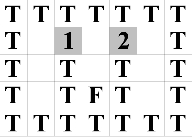
\includegraphics[width=0.22\textwidth]{woods101a}}\hfill
  \subfigure[Sensory configuration of the two aliasing positions]{
  	\label{figure:woods101b}
  	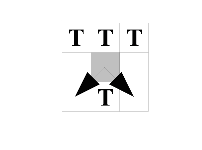
\includegraphics[width=0.22\textwidth]{woods101b}}\hfill
  \caption{\mathversion{bold}The \emph{Woods101} environment: Trees are marked with $T$, food is marked with $F$.}
  \label{figure:woods101}
\end{figure}

However, some Maze problems offer perceptually identical situations that require different actions to reach the food. This problem is often studied in the context of \emph{non-Markov environments}. \emph{Woods101} (see Figure~\ref{figure:woods101a}) is a typical example of a \emph{partially observable Markov decision process (POMDP)}, where an animat cannot distinguish different situations due to a lack of global environmental information. 

The animat is placed in a free random field (it can sense the eight adjacent cells) and has to learn to reach the food denoted with $F$, while trees $T$ blocking any movement. Here, the aliasing positions, marked with 1 and 2, share the same sensory configuration, but require different optimal actions (see Figure~\ref{figure:woods101b}, each optimal action for the different positions is marked with an arrow). In position 1, the optimal action is to move to the bottom right, while the optimal action in position 2 is to move to the bottom left. Thus, an XCS cannot evolve an optimal policy for \emph{Woods101} (without further modifications). Using records of past condition-action-mappings by adding temporary memory is a common approach to cope with such environments, see \cite{Lan98,LW00}.

A second non-Markov property is still embedded in \emph{multi-agent} environments and this is related to a change of an agent's internal state. In scenarios with more than one learning agent, an agent has to evaluate actions that may be caused by its own internal state or that are the result of other agent's actions. It is difficult to recognize an environmental change, which is caused by the change of another agent's internal state, due to a lack of the other agent's information. Even if an agent stays in the same location, the agent cannot evaluate the environmental changes. Moreover, memory-based approaches will fail, since any memory, which stores information about the environment, becomes invalid after each step. This second non-Markov property is often defined as a \emph{non-observable Markov decision process (NOMDP)}, see~\cite{TTS01}.

As shown in Section~\ref{subsection:scenario-classification}, the predator/prey scenario, presented in the following and used as testbed in this paper, includes both non-Markov properties (POMDP and NOMDP). Thus, learning in such environments is more complex than learning in single-agent environments (where only one agent adapts to its dynamically changing environment) and requires a different approach, as discussed in Section~\ref{section:the-reward-function}.

\subsection{The Predator/Prey Example}
\label{section:the-predator-prey-example}

The predator/prey domain, introduced by \cite{BJD86}, is an appropriate multi-agent example that has successfully been studied in a variety of instantiations \cite{SV00}. It does not serve as a complex real world domain, but as a test scenario for demonstrating and evaluating manifold research ideas. % Introduced by \cite{BJD86}, researchers have investigated different instantiations of its original formulation in the context of different application areas \cite{SV00}. 
Both, predator and prey, typically can move into four different directions -- north, east, south, and west. Mostly, predators follow a capturing strategy as a goal, while the prey randomly moves or stays still with a certain probability in order to simulate slower movements than the predators. A variation is that the prey moves faster than the predators. In this case, a strategic collaborative effort is required by the predators. An active escaping strategy, where the prey adapts and learns its behavior, may also be possible.
% Worlds with other shapes as spaces (e.\,g., squares) or continuous/toroidal worlds without edges (predators and prey can move off one end of the world and come back on another end) are possible. 
% The predators try to capture the prey in such a way that the prey cannot move to an unoccupied position. If the grid world has edges, it might be possible that fewer than four predators can catch the prey by surrounding the prey against an edge of obstacles or in a corner of the world. Other parameters of the predator/prey domain are: Do the agents move simultaneously or successively -- one after the other? Is the local view of an agent limited or does an agent see the whole environment? And last, but not least, is direct communication between the agents allowed?
While predators and prey(s) have limited actions and follow well defined objectives, the predator/prey domain is simple to understand, easy to implement, and flexible enough to demonstrate a range of different scenarios. % , which have been emerged over the past decades. % The general approach of the predator/prey example, the possibility to customise and adopt the scenario to manifold applications, or the wide\-spread experience that is documented, not only in multi-agent literature, result in the assumption that the predator/prey example can be used as a valid and flexible testbed for technical OC scenarios.
Here, a simple instantiation of the predator/prey scenario is examined. 
%, where the predators fulfill a \emph{cooperative observation task} and are rewarded for just being very close to the prey. Thus, it is not necessary to surround and catch the prey, the predators try to observe the prey as long as possible.
% For the predators to fulfill the \emph{cooperative observation task} it is not necessary to surround and catch the prey, they are rewarded for the amount of time just being very close to it.
Predators fulfill a \emph{cooperative observation task}, where agents can sense other agents, but not communicate with each other. Then, predators are rewarded for the amount of time just being very close to the prey (i.\,e., it is not necessary to surround and catch it). 

\subsection{Classification of the Example}
\label{subsection:scenario-classification}

Environments can be classified as an MDP, an POMDP, or an NOMDP. The main characteristics of the predator/prey scenario, which is here investigated, could be summarized as follows:

\begin{enumerate*}
	\item An agent has only access to local information,
	\item the whole field usually consists of open areas with randomly placed obstacles,
	\item each agent has an internal state unknown to others,
	\item the scenario is dynamic (agents act in parallel),
	\item the agents (i.\,e., the predators) share and cooperatively contribute to a glo\-bal observation task, and
	% \item the scenario runs continuously.
	\item the global observation task forces continuous agents' activities.  
\end{enumerate*}

It is obvious that the three scenarios, as intended in Figure~\ref{figure:scenarios}, constitute being no MDPs, since agents' sensory information is limited (1, 3) and different positions share the same sensory configuration (2). Moreover, adding the capability of storing information would not restore the Markov property (4), as demonstrated on \emph{Woods101} in \cite{Lan98,LW00}. This let us conclude that the scenarios could not be any POMDPs. Finally, this also remains that the scenarios have to be NOMDPs. 

Additionally, if each predator tries to learn its cooperative behavior using an XCS, a clearly defined (local) goal (5) will be needed to generate payoffs, when agents have reached their goals. Furthermore, a typical multi-step XCS scenario will be restarted, if an agent has reached its goal. But, the observation task is a continuous task (6). % In addition, special care is needed when applying XCS as is no clear local goal (5) and the scenario is not restarted when reaching the global goal (6). 
To conclude, a different approach is needed. Thus, a modified multi-step XCS variant is introduced in the following that can properly handle these issues.

In XCS literature, NOMDP environments are discussed in \cite{Miyazaki2,TTS01}. There, the issue of non-observability is either investigated by a very simplified scenario with only two agents or by establishing complex communication and centralized organization mechanisms, where all agents share and contribute to a global LCS with global information. Both approaches seem not applicable here, since the investigated scenarios focus on more than two agents and (global) communication between the predators has not been intended. Thus, new mechanisms are required to learn this % cooperative 
collaborative and dynamic observation task using the XCS algorithm. The most important step to solve this problem is the design of an adequate, \emph{cooperative reward function}. % , as discussed in the following. % which is discussed in the following section.
